\chapter{System Requirements}
\label{chptr:system_requirements}

A system that is used in the context of ETCS to operate a train must be dependable.
Dependability is a characteristic for computing systems to ''deliver [a] services that can justifiably be trusted''~\cite{AvizienisDependability2001}.
It includes properties such as reliability, maintainability and safety.
Based on the definition by IEEE 610.12-1990, reliability is "the ability of a system or component to perform its required function under stated conditions for a specified period of time"\cite{ieee610.12}.
A safe system is in a condition where the number of failures is small~\cite{HollnagelSafety}.
In other words, safety is defined as a system's probability to not have any failures that would lead to a serious outcome in a specified time span~\cite{GeffroyMotetDependableComputing}.
The serious outcome depends on the execution environment and is often linked to a catastrophic failure.
\\

In this chapter, requirements for dependable systems and ways to measure these requirements are presented.
The requirements, definitions, and evaluation methods build the foundation for a system evaluation.

\section{Requirement}
\todo{Write more about requirements}
- Be concrete about requirements
	- What should the system do
		- Linking via RBC, Balise Telegram, Filtering, Konsistency testing
		- Open Stack (Each component should be capable of replacing any other component)
		- Self checking in the system
	- How reliable, how safe

\section{•}


% Maybe also cover testability?

\section{Reliability}

Reliability can be mathematically defined as a function of time which expresses the probability that a system is operating as specified at a time $t_1$, given that it was operating as specified at time $t | t \leq t_1$.
One important characteristic of reliability is that it does not increase over time.
For hardware devices, reliability decreases over time due to abrasion while it stays constant for software.
This is because hardware devices are exposed to external influences, such as temperature or vibration~\cite{GeffroyMotetDependableComputing}.

In this work, the exact environmental influences are not known.
Therefore, the reliability evaluation will be made on mathematical reliability models that base on reliability parameters deduced from the applied components and the expected environment.

\subsection{Reliability Models}
Geffroy an Motet present two reliability models, namely the exponential law and the Weinbull law, but argue that the exponential law is most commonly used for electronic systems~\cite{GeffroyMotetDependableComputing}.

The exponential law describes a component's reliability as an exponential function.
\begin{equation}
R(t) = e^{-\lambda t}.
\label{eq:expFailureLaw}
\end{equation}
As described above, a system's reliability by definition decreases over time, which is expressed in~\autoref{eq:expFailureLaw}.
The parameter $\lambda$ encodes the probability of failures occuring in a certain time span.
During this work, the value for $\lambda$ is considered to be constant, although in practice it would change over time following a \texttt{bathtub courve}~\cite{GeffroyMotetDependableComputing}.

In order to make use of the exponential failure law, Berry W. Johnson proposes two analytical techniques for analyzing a system's reliability, namely combinatorial modeling and Markov modeling~\cite{BarryFaultToleranceAnalysis}.
He argues that, while in serial systems each element needs to operate in the prescribed way for the system to be reliable, in parallel systems only a subset of all components needs to function correctly.

\paragraph{Serial System}
A serial system is a system that contains no redundancy~\cite{BarryFaultToleranceAnalysis}.
Thus, the reliability of a serial system is directly dependent on the propability that all individual components work correctly.
%Therefore, the reliability of a serial system, consisting of $N$ individual components, at time $t$ can be calculated as
%\begin{equation}
%R_s(t) = P\{ R_1(t) \cap R_2(t) \cap \dots \cap R_N(t) \}
%\end{equation}
%where $R_s(t)$ describes the reliability of the entire serial system at time $t$ and $R_i(t)$  being the probability of component $C_i$ working correctly at time $t$.
For independent components, which follow the exponential failure law, holds~\cite{BarryFaultToleranceAnalysis}:
\begin{equation}
R_s(t) = e^{\sum_{i = 1}^N \lambda_i t}
\label{eq:combReliabSerial}
\end{equation}

\paragraph{Parallel System}
In a parallel system, as defined by Johnson, where $N$ identical components are working in parallel, only one individual component is required to work correctly for the entire system to work correctly.
A parallel system's reliability is therefore reciprocal to the probability of all $N$ components failing at the same time.
%
%This is expressed through
%\begin{equation}
%R_p(t) = P\{ R_1(t) \cup R_2(t) \cup \dots \cup R_n(t) \}
%\end{equation}
%where $R_p(t)$ being the reliability of the entire parallel system at time $t$ and $R_i(t)$ being the probability of component $C_i$ working correctly at time $t$.
When all $C_i(t)$ are independent and follow the exponential law, a parallel system's reliability is expressed through~\cite{BarryFaultToleranceAnalysis}:
\begin{equation}
R_p(t) = \sum_{i = 1}^N ( e^{-\lambda t} ) - \prod_{i = 1}^N e^{-\lambda t}
\label{eq:combReliabParallel}
\end{equation}

A generalization of parallel systems is provided by \gls{MOON}-systems.
Such systems require $M$ out of $N$ components in a system to work correctly for the entire system to be considered reliable.
This behavior is expressed in
\begin{equation}
R_{moon}(t) = \sum_{i = M}^N {N \choose i} * (e^{-\lambda t})^i * (1 - e^{-\lambda t})^{N - i}
\label{eq:reliabilityMOON}
\end{equation}
with ${N \choose M}$ being the binominal coefficient and the system's components follow the exponential failure law.

For the reliability in \gls*{MOON} systems applies:

\begin{hypothesis}
Increasing the number of replicas $N$ while keeping the number of required replicas to agree on a value $M$ constant, cannot decrease a system's reliability.
\label{hyp:NIncreaseMConstant}
\end{hypothesis}

\begin{hypothesis}
Decreasing the number of required replicas to agree on a value $M$ while keeping the number of replicas $N$ constant, cannot decrease a system's reliability.
\label{hyp:MDecreaseNConstant}
\end{hypothesis}

\autoref{hyp:NIncreaseMConstant} and \autoref{hyp:MDecreaseNConstant} can be shown through induction:

\paragraph{Proof of~\autoref{hyp:NIncreaseMConstant}}
Let $M$ be contant and $M \leq N$, let $R_{c}$ the reliability of the system's components.

\subparagraph{Begin of Induction}
Let $N = 1 \Rightarrow M = 1$.\\
$R_{1oo1} = {1 \choose 1} * R_{c}^1 * (1 - R_{c})^0 = R_{c}$

\subparagraph{Induction Hypothesis}
$R_{MooN}$ describes the reliability for a M-out-of-N-system and a components reliability $R_{c}$ can only be positive.

\subparagraph{Induction Step}
$R_{MooN+1} = \sum_{i=M}^{N+1} {N + 1 \choose i} * R_{c}^i * (1 - R_c)^{N + 1 - i}$\\
$= \sum_{i=M}^{N} {N \choose i} * R_{c}^i * (1 - R_c)^{N - i} + {N+1 \choose N+1} * R_c^{N+1} * (1 - R_c)^{N+1 - N+1}$\\
$= R_{MooN} + R_c^{N+1}$ \\
$\Rightarrow R{MooN} \leq R_{MooN+1}$\\
$\square$


\paragraph{Proof of~\autoref{hyp:MDecreaseNConstant}}
Let $N$ be constant and $N \geq N$, let $R_c$ be the reliability of a system's component.

\subparagraph{Begin of Induction}
Let $M = 1 \Rightarrow N = 1$.\\
$R_{1oo1} = {1 \choose 1} * R_{c}^1 * (1 - R_{c})^0 = R_{c}$

\subparagraph{Induction Hypothesis}
$R_{MooN}$ describes the reliability for a M-out-of-N-system and a components reliability $R_{c}$ can only be positive.

\subparagraph{Induction Step}
$R_{M-1ooN} = \sum_{i=M-1}^{N} {N \choose i} * R_{c}^i * (1 - R_c)^{N - i}$\\
$= {N \choose M-1} * R_c^{M-1} * (1 - R_c)^{N - M-1} + \sum_{i=M}^{N} {N \choose i} * R_{c}^i * (1 - R_c)^{N - i}$\\
$= {N \choose M-1} * R_c^{M-1} * (1 - R_c)^{N - M-1} + R_{MooN}$\\
$\Rightarrow R_{M-1ooN} \geq R_{MooN}$\\
$\square$

The drawback of \autoref{eq:combReliabSerial} and \autoref{eq:combReliabParallel} are, that they imply the component's reliability characteristics to be independent.
This holds for individual faults such as random hardware failures, but not for external or common faults such as common core errors or external distrubances.
Therefore, the combinatorial reliability modelling described above can only be used when considering independent faults such as random hardware errors~\cite{BarryFaultToleranceAnalysis}.
In order to make the combinatorial approach more applicable, diverse replicas or independen power supplies can be used.
\todo{Find definition for diverse redundancy}
\todo{Find more examples how to make the nodes more independent}


%In order to model the reliability of more complex systems and to also express reliability in presence of fault mitigation and repair mechanisms, Markov models can be used.
%In the Markov model, state and state transitions are evaluated.
%For reliability inspection, the states represent a combination of faulty and non-faulty components.
%The state transitions encode events in which components fail in the system.
%Each state transition is associated with a probability that can express properties such as the probability of failure and the probability of fault mitigation or fault recovery.

As shown in \todo{Ref}, the system's reliability cannot decrease when keeping the number of replicas constant but decreasing the required number of replicas to agree on a value.
This is because it allows more replicas to fail in order for the system to still produce valid outputs.

\section{Safety}
A form of expressing a system's safety is \gls*{SIL}.
The \gls*{SIL} of a system is defined as the probability that a system cannot respond to a potentially dangerous condition~\cite{SallekSIL}.
An important distinction between a safe and a reliable system is, that a safe system are allowed to fail as long as they do not lead to a serious outcome.

A system that is designed to remain safe in presence of occasional failures is defined to be fault tolerant~\cite{RandellFaultTolerance}.
In order for systems to be fault tolerant, the failure has to be detected and identified beforhand in a \gls*{FDI} process.
A \gls*{FDI} process consists of two stages to detect failures on a system's output~\cite{ChowFailureDetectionSystems}.
In a first step, by Chow and Willsky called \textit{residual} stage, a deviation between the expected and actual output are determined.
This deviation factor is called the output's \textit{residuals}.
In order for the residual stage to function, the components that are determining the residuals have to know about the system's normal behavior.
In a second phase, called the \textit{decision} state, a decision function is applied on the residuals to detect the presence of failures.

\section{Distributed Systems}

One way of building a dependable system, even out of undependable components, is through distribution (Source ReliabilityEngineering Slides).
This is because, in general, the failure of one individual component in a distributed system does not affect the remaining component's dependability.
However, if the failing component was responsible for a crucial system function, then a single failure can lead to a failure of the entire system.
A commonly applied technique for maintaining a system's functionality even when a crucial componant fails is redundancy~\cite{TanenbaumSteen07}.
Therefore, the crucial component's work is performed on multiple components, called replicas, simultaneously.
When one of the crucial components fails, the remaining replicas still allow the system to continue its work.

In the following of this chapter, different distributed and redundant system architecture approaches are described and assessed based on~\todo{Woran?}.
Later, methods for facilitating failure detection and fault tolerance in distibuted and redundant systems are introduced.
All this is done with the aim of building a highly safe \gls*{SIL} 4 system.
At first, however, fundamental terms and building blocks are described.

\subsection{Redundancy}
A frequently used pattern for facilitating a higher dependency is redundancy~\cite{GeffroyMotetDependableComputing}.
However, adding redundancy also increases the complexity as well as design and building costs of a system.

In computing systems, the two types \texttt{functional}- and \texttt{structural}-redundancy can be found.
While functional-redundancy incorporates a system's external manner, structural-redundancy refers to its internals.

\subsubsection{Functional Redundancy}
Functional redundancy is encoded in the relationship between a system's input and its output.
It allows the system to filter out impossible or unacceptable inputs or outputs.
Functional redundancy is independent of the system's design and implementation and solely depends on its functions.
A way of adding functional redundancy to a system is to structure it into interconnected modules~\cite{GeffroyMotetDependableComputing}.
\todo{Explain this further}

\subsubsection{Structural Redundancy}
For structural redundancy, additional components are added to the system that would be unnecessary, provided all components are working correctly.
Structural redundancy can be applied in software, in hardware or in the time domain~\cite{GeffroyMotetDependableComputing}.
Examples for structural redundancy are:

\paragraph{Standby Redundancy}
In standby redundancy, the redundant components are subdevided into primary and secondary components.
A third component type is required to switch between the primary and secondary components, when required.
The switching step, however, is not possible without any costs and adds an additional point of failure~\cite{PepperlFuchs}.
Standby redundancy is subdevided into cold and hot standby, implicated whether the secondary components are turned off or on while they are not used.

\paragraph{M-out-of-N Redundancy}
Another popular redundancy pattern for industrial applications is \gls*{MOON}-redundancy~\cite{GamerIncreasingMOON}.
Thereby, N individual components are executing the same task simultaneously and all separate outputs are collected.
The system finally generates the overall output by selecting the value where at least M out of the N components agreed on.
This allows the system to generate the right output even if $N-M$ components produced a wrong output.



\todo{Define module composition}

In structural redundant systems, it often happens that multiple redundant outputs need to be reduced to a single system output.
In order to produce a single output out of $N$ individual outputs, a voter or a consensus algorithm could be used.

\paragraph{Voter} 
A voter is an entity that collects the components individual outputs and performs a voting algorithm to combine them to a single output.
The voter approach has the benefit that it is fast and easy to implement.
For voter based systems, Chow and Willsky argue that system output's residual generation can be done by simply comparing outputs of redundantly working components~\cite{ChowFailureDetectionSystems}.
However, a voter is a single point of failure and thereby impairs the entire systems reliability and availability.

\paragraph{Consensus} 
A consensus algorithm is applied to reach consensus among the system's individual components in order to agree on a single output value.
This single output value is required to be proposed by at least one component~\cite{lamport2001paxos}.
While not having a single point of failure anymore, consensus approaches typically introduce a communication overhead and lead to rigid configurations~\cite{GamerIncreasingMOON}.


\section{Choosing a System Architecture}

\begin{figure}[!hb]
	\centering
	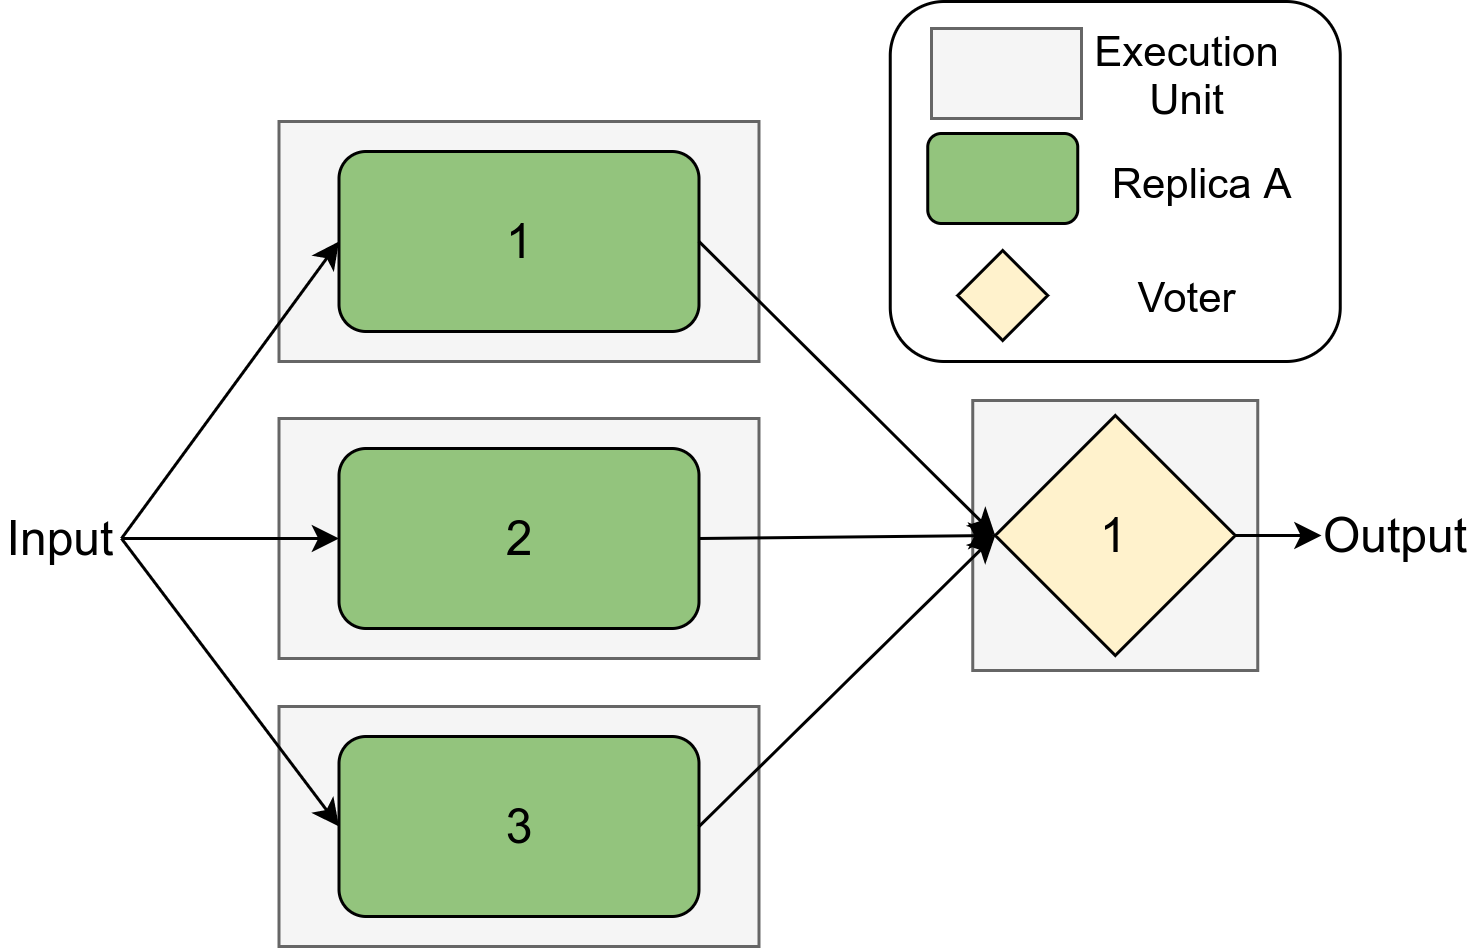
\includegraphics[width=0.75\linewidth]{images/Classical2OO3}
	\caption{Classical 3-out-of-2 redundancy, also known as \Gls*{TMR}.}
	\label{fig:Classical2OO3}
\end{figure}

\autoref{fig:Classical2OO3} depicts a 2-out-of-3 redundancy pattern, where three replicas are preforming the same work in parallel.
A voter collects the individual outputs and reduces them to a single system output.
The system output must qualify the characteristic that at least two out of the three replicas agree on this output.
All replicas, as well as the voter, are running on individual execution units.

It is assumed that all replicas follow the exponential failure law.
Based on \autoref{eq:expFailureLaw} and \autoref{eq:reliabilityMOON} follows for the replicas reliability
\begin{equation}
R_{2oo3}(t) = \sum_{i = 2}^3 {3 \choose i} * (e^{-\lambda t})^i * (1 - e^{-\lambda t})^{3 - i}
\end{equation}

Throughput can be increased by combining the parallel and serial pattern in a pipelined way.
This also has the way that it adds functional redundancy to the system~\cite{GeffroyMotetDependableComputing}.



%\section{Redundancy Pattern Discussion}
%As described above, there exist two categories of redundant architectures that are evaluated here, namely voter-based and consensus-based redundancy.
%All presented architectures in this section will be evaluated based on failure probability, fault tolerance, reliability, and availability.
%In this case, the system's reliability can be derived from a combination of its failure probability and fault tolerance.
%The system's availability is defined as the quantity of time the system is functioning as it should.
%By implication, the system is unavailable when it does not work as intended but a safe state is taken.
%When the system is unavailable and in an unsafe state, it is considered to be unreliable.
%The method \texttt{analytical redundancy}, for identifying the fault tolerance in the redundant system, as proposed by Chow and Willsky, will be used~\cite{ChowFailureDetectionSystems}.

%\subsection{Classical M-out-of-N Redundancy}
%The example shown in \todo{figure 1} depicts 2-out-of-3 redundancy, also known as triple-modular redundancy.
%Three replicas are performing the same work in parallel and the voter requires at least two identical outputs from the replicas to perform a majority voting.



% Bewertungskriterien
% - Ausfallwahrscheinlichkeit mit Markov Model
% - Fault tolerance
% - Failure rate
% - Repair rate
% - Mean time to failure
% - Mean time between failure
% - Mean time to recovery
% - Availability